\section{Evaluation}
\label{sec:evaluation}

We evaluate our enclave framework with respect to
security (\S~\ref{sec:security}),
financial cost (\S~\ref{sec:cost}), and performance.  As for performance, we
study the rate at which one can generate
attestation documents (\S~\ref{sec:attestation-performance}) and
measure end-to-end request latency and throughput (\S~\ref{sec:end-to-end}).

\subsection{Security Considerations}
\label{sec:security}

There are three key components to the overall security of enclave applications;
(\emph{i}) Amazon's Nitro enclave system itself, (\emph{ii}) our framework, and
(\emph{iii}) the application that runs on top of our framework.

The very foundation of our framework's security lies in the soundness of the
design of Nitro enclaves.  While Amazon published the conceptual design, the
concrete hardware and software implementation remains confidential.  The
decision to allocate physically separate resources to enclaves appears promising
but only time will tell if Nitro enclaves can resist the types of attacks that
have been plaguing SGX.  If we assume that Nitro enclaves are acceptably
secure, the next critical layer is our software framework.

A significant security aspect of our framework is its size; it is well
understood that complexity is the enemy of security.  Our framework counts less
than 700 lines of code and has four direct dependencies that are not maintained
by either us or the Go project.\footnote{The dependencies are chi~\cite{chi}
(provides an HTTP request router), nsm~\cite{nsm} (provides an interface to
interact with the Nitro hypervisor), vsock~\cite{vsock} (provides an API for the
VSOCK address family), and tenus~\cite{tenus} (provides an API to configure
Linux's networking devices).}  Four is worse than zero, but is still manageable
and reasonably easy to audit in its entirety.  We believe that our choice of
using Go and the deliberately small trusted computing base greatly reduces---but
does not eliminate!---the attack surface.

The highest layer in the software stack is the enclave application itself.  The
biggest security threat are side channel attacks and programming bugs---both
unintentional and intentional.  It is the application developer's
responsibility to prevent side channel attacks and write bug-free code.  As we
pointed out in Section~\ref{sec:limitations}, programming bugs can be
intentional, i.e., the service provider may deliberately introduce bugs that
leak sensitive information.  From the user's point of view, eternal vigilance
is therefore the price of security.

\subsection{Financial Cost}
\label{sec:cost}

Nitro enclaves do not incur any extra cost in addition to what the underlying
EC2 host costs---they can be considered a ``free'' extension to EC2.  Nitro
enclaves are however only available for select types of EC2 instances because
they require their own CPU and a minimum amount of memory, and those instance
types are pricier than the lowest tier that AWS offers.

We are currently working on deploying the IP address pseudonymization prototype
that we introduced in Section~\ref{sec:pseudonymization}.  We estimate that our
enclave is going to have to handle an average of 5,000 requests per minute,
coming from more than ten million clients.  Our test deployment uses a single
c5.xlarge EC2 host in the U.S. East region which costs \$0.17 per hour to
operate, amounting to approximately \$125 per month.

\subsection{Attestation Documents}
\label{sec:attestation-performance}

The fetching of attestation documents is a critical part of our framework's
overall performance.  We wrote a stress test tool that requests as many
attestation documents as it can over sixty seconds.  The tool is essentially a
minimal enclave application that requests attestation documents in a loop.  For
each attestation document, we asked the hypervisor to include an incrementing
nonce, to avoid any speedups by caching.  We were able to obtain approximately
900 documents per second, with each request taking a median of one millisecond
($s = 0.3\,\text{ms}$) to fetch the attestation document.\footnote{We performed
our measurements on a c5.xlarge EC2 host which comes with four CPUs and eight
GiB of memory.}

\subsection{Application Latency and Throughput}
\label{sec:end-to-end}

Next, we set out to measure the networking latency of the critical path, as
illustrated in Figure~\ref{fig:stress-test}.  In particular, we test the
latency of our TCP proxy, the VSOCK interface between EC2 and enclave, and a
minimal enclave application.
%
We measure latency in three separate setups, designed to help us understand how
much latency each component in our data flow adds:

\begin{figure}[t]
    \centering
    \begin{tikzpicture}[node distance=20pt]
  \node [draw,
         label={[anchor=north]above:EC2 host},
         minimum height=40pt,
         align=center,
         minimum width=110pt] (ec2) {};

  \node [draw,
         label={[anchor=north]above:Enclave},
         right=0pt of ec2,
         fill=black!10,
         minimum height=40pt,
         minimum width=120pt] (enclave) {};

  \node [draw,
         align=center,
         yshift=-5pt,
         left=10pt of ec2.east] (proxy) {Proxy};

  \node [draw,
         align=center,
         left=of proxy] (baton) {Baton};

  \node [draw,
         align=center,
         fill=white,
         yshift=-5pt,
         right=10pt of enclave.west] (nitriding) {Nitriding};

  \node [draw,
         align=center,
         fill=white,
         right=of nitriding] (app) {Web srv};

  \node [xshift=15pt,
         yshift=-5pt,
         align=center] at (enclave.north west)
    {\footnotesize \color{gray} VSOCK};

  % Baton talking to the Web service.
  \draw[-latex] ([yshift=5pt]baton.east) -- ([yshift=5pt]proxy.west);
  \draw[-latex] (baton.east) -- (proxy.west);
  \draw[-latex] ([yshift=-5pt]baton.east) -- ([yshift=-5pt]proxy.west);

  \draw[-latex] ([yshift=5pt]proxy.east) -- ([yshift=5pt]nitriding.west);
  \draw[-latex] (proxy.east) -- (nitriding.west);
  \draw[-latex] ([yshift=-5pt]proxy.east) -- ([yshift=-5pt]nitriding.west);

  \draw[-latex] ([yshift=5pt]nitriding.east) -- ([yshift=5pt]app.west);
  \draw[-latex] (nitriding.east) -- (app.west);
  \draw[-latex] ([yshift=-5pt]nitriding.east) -- ([yshift=-5pt]app.west);

\end{tikzpicture}

    \caption{Our stress test tool tests the performance of our critical path,
    consisting of the TCP proxy, the VSOCK interface, and Go's HTTP stack in
    the enclave application.}
    \label{fig:stress-test}
\end{figure}

\begin{description}
  \item[Full:] This represents the full data flow as it would occur in
    production, i.e. client $\rightarrow$ TCP proxy $\rightarrow$ VSOCK
    interface $\rightarrow$ enclave application.

  \item[No proxy:] This setup does not contain the TCP proxy, i.e., the client
    talks to the VSOCK interface directly, i.e. client $\rightarrow$ VSOCK
    interface $\rightarrow$ enclave application.

  \item[Direct:] This setup does not contain the TCP proxy and the VSOCK
    interface.  Instead, the client directly talks to an application instance that is
    running \emph{outside} the enclave, i.e., client $\rightarrow$ application.
\end{description}

As part of our measurement setup, We first deploy the code from
Figure~\ref{fig:hello-world}---a minimalistic application that responds with
the string ``hello world'' upon receiving requests for the path /hello-world.
It's important to use a minimalistic application because we're only interested
in the latency that is caused by the components \emph{before} a request reaches
the enclave application.

To simulate clients, we use the HTTP load test tool Baton~\cite{baton}.  We run
Baton on the parent EC2 host and instruct it to send as many requests to the
TCP proxy as possible within 30 seconds, using 50 concurrent threads.  We had to
patch Baton's source code to add VSOCK support (to be able to send requests
directly to the enclave via the VSOCK interface) and to log latency
percentiles.  Note that our measurements constitute a \emph{lower bound} of the
latency that is achievable.  Real-world applications will exhibit higher latency
because clients send their requests over the Internet (which adds considerable
networking latency) and the enclave application is likely to be more complex
(which adds computational latency).

Figure~\ref{fig:latency-msmts} illustrates the results for our three test
setups.  The full pipeline is able to sustain 7,500 requests per second, with a
mean latency of 12.7 milliseconds.  Removing the proxy nearly doubles the
requests to 14,100 per second and lowers the mean latency to 6.5.  Finally, a
direct connection to the application---without proxy and VSOCK interface--once
again nearly doubles the number of requests, reaching 27,900 per second, with a
mean latency of only 3.2 milliseconds.  Figure~\ref{fig:latency-cdf} shows the
empirical CDF of the same latency measurements for our three test setups.

\begin{figure}[t]
    \centering
    \begin{tabular}{l r r r}
    \toprule
      Setup & Reqs/sec & Mean lat. (ms) & Max lat. (ms) \\
    \midrule
    Full & 7,500 & 12.7 & 56.0 \\
    No proxy & 14,100 & 6.5 & 52.0 \\
    Direct & 27,900 & 3.2 & 50.0 \\
    \bottomrule
    \end{tabular}
    \caption{Using 100 concurrent requests and 100,000 requests in total.}
    \label{fig:latency-msmts}
\end{figure}


\begin{figure}[t]
    \centering
    % Created by tikzDevice version 0.12.3.1 on 2023-01-22 18:15:41
% !TEX encoding = UTF-8 Unicode
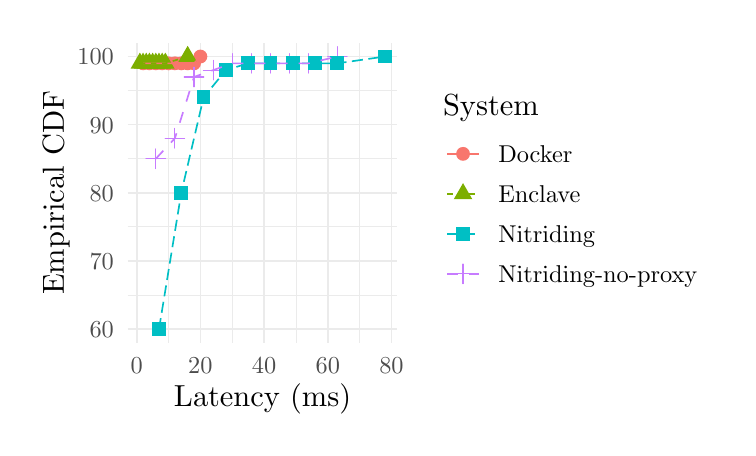
\begin{tikzpicture}[x=1pt,y=1pt]
\definecolor{fillColor}{RGB}{255,255,255}
\path[use as bounding box,fill=fillColor,fill opacity=0.00] (0,0) rectangle (252.94,144.54);
\begin{scope}
\path[clip] ( 36.11, 30.69) rectangle (133.59,139.04);
\definecolor{drawColor}{gray}{0.92}

\path[draw=drawColor,line width= 0.3pt,line join=round] ( 36.11, 47.92) --
	(133.59, 47.92);

\path[draw=drawColor,line width= 0.3pt,line join=round] ( 36.11, 72.55) --
	(133.59, 72.55);

\path[draw=drawColor,line width= 0.3pt,line join=round] ( 36.11, 97.18) --
	(133.59, 97.18);

\path[draw=drawColor,line width= 0.3pt,line join=round] ( 36.11,121.80) --
	(133.59,121.80);

\path[draw=drawColor,line width= 0.3pt,line join=round] ( 50.90, 30.69) --
	( 50.90,139.04);

\path[draw=drawColor,line width= 0.3pt,line join=round] ( 73.92, 30.69) --
	( 73.92,139.04);

\path[draw=drawColor,line width= 0.3pt,line join=round] ( 96.94, 30.69) --
	( 96.94,139.04);

\path[draw=drawColor,line width= 0.3pt,line join=round] (119.95, 30.69) --
	(119.95,139.04);

\path[draw=drawColor,line width= 0.6pt,line join=round] ( 36.11, 35.61) --
	(133.59, 35.61);

\path[draw=drawColor,line width= 0.6pt,line join=round] ( 36.11, 60.24) --
	(133.59, 60.24);

\path[draw=drawColor,line width= 0.6pt,line join=round] ( 36.11, 84.86) --
	(133.59, 84.86);

\path[draw=drawColor,line width= 0.6pt,line join=round] ( 36.11,109.49) --
	(133.59,109.49);

\path[draw=drawColor,line width= 0.6pt,line join=round] ( 36.11,134.11) --
	(133.59,134.11);

\path[draw=drawColor,line width= 0.6pt,line join=round] ( 39.39, 30.69) --
	( 39.39,139.04);

\path[draw=drawColor,line width= 0.6pt,line join=round] ( 62.41, 30.69) --
	( 62.41,139.04);

\path[draw=drawColor,line width= 0.6pt,line join=round] ( 85.43, 30.69) --
	( 85.43,139.04);

\path[draw=drawColor,line width= 0.6pt,line join=round] (108.45, 30.69) --
	(108.45,139.04);

\path[draw=drawColor,line width= 0.6pt,line join=round] (131.46, 30.69) --
	(131.46,139.04);
\definecolor{fillColor}{RGB}{248,118,109}

\path[fill=fillColor] ( 41.69,131.65) circle (  2.50);

\path[fill=fillColor] ( 43.99,131.65) circle (  2.50);

\path[fill=fillColor] ( 46.30,131.65) circle (  2.50);

\path[fill=fillColor] ( 48.60,131.65) circle (  2.50);

\path[fill=fillColor] ( 50.90,131.65) circle (  2.50);

\path[fill=fillColor] ( 53.20,131.65) circle (  2.50);

\path[fill=fillColor] ( 55.50,131.65) circle (  2.50);

\path[fill=fillColor] ( 57.81,131.65) circle (  2.50);

\path[fill=fillColor] ( 60.11,131.65) circle (  2.50);

\path[fill=fillColor] ( 62.41,134.11) circle (  2.50);
\definecolor{fillColor}{RGB}{124,174,0}

\path[fill=fillColor] ( 40.54,135.54) --
	( 43.91,129.71) --
	( 37.18,129.71) --
	cycle;

\path[fill=fillColor] ( 41.69,135.54) --
	( 45.06,129.71) --
	( 38.33,129.71) --
	cycle;

\path[fill=fillColor] ( 42.84,135.54) --
	( 46.21,129.71) --
	( 39.48,129.71) --
	cycle;

\path[fill=fillColor] ( 43.99,135.54) --
	( 47.36,129.71) --
	( 40.63,129.71) --
	cycle;

\path[fill=fillColor] ( 45.15,135.54) --
	( 48.51,129.71) --
	( 41.78,129.71) --
	cycle;

\path[fill=fillColor] ( 46.30,135.54) --
	( 49.66,129.71) --
	( 42.93,129.71) --
	cycle;

\path[fill=fillColor] ( 47.45,135.54) --
	( 50.81,129.71) --
	( 44.08,129.71) --
	cycle;

\path[fill=fillColor] ( 48.60,135.54) --
	( 51.96,129.71) --
	( 45.23,129.71) --
	cycle;

\path[fill=fillColor] ( 49.75,135.54) --
	( 53.11,129.71) --
	( 46.39,129.71) --
	cycle;

\path[fill=fillColor] ( 57.81,138.00) --
	( 61.17,132.17) --
	( 54.44,132.17) --
	cycle;
\definecolor{drawColor}{RGB}{199,124,255}

\path[draw=drawColor,line width= 0.4pt,line join=round,line cap=round] ( 42.76, 97.18) -- ( 49.83, 97.18);

\path[draw=drawColor,line width= 0.4pt,line join=round,line cap=round] ( 46.30, 93.64) -- ( 46.30,100.71);

\path[draw=drawColor,line width= 0.4pt,line join=round,line cap=round] ( 49.67,104.56) -- ( 56.73,104.56);

\path[draw=drawColor,line width= 0.4pt,line join=round,line cap=round] ( 53.20,101.03) -- ( 53.20,108.10);

\path[draw=drawColor,line width= 0.4pt,line join=round,line cap=round] ( 56.58,126.73) -- ( 63.64,126.73);

\path[draw=drawColor,line width= 0.4pt,line join=round,line cap=round] ( 60.11,123.19) -- ( 60.11,130.26);

\path[draw=drawColor,line width= 0.4pt,line join=round,line cap=round] ( 63.48,129.19) -- ( 70.55,129.19);

\path[draw=drawColor,line width= 0.4pt,line join=round,line cap=round] ( 67.01,125.66) -- ( 67.01,132.72);

\path[draw=drawColor,line width= 0.4pt,line join=round,line cap=round] ( 70.39,131.65) -- ( 77.45,131.65);

\path[draw=drawColor,line width= 0.4pt,line join=round,line cap=round] ( 73.92,128.12) -- ( 73.92,135.18);

\path[draw=drawColor,line width= 0.4pt,line join=round,line cap=round] ( 77.29,131.65) -- ( 84.36,131.65);

\path[draw=drawColor,line width= 0.4pt,line join=round,line cap=round] ( 80.82,128.12) -- ( 80.82,135.18);

\path[draw=drawColor,line width= 0.4pt,line join=round,line cap=round] ( 84.20,131.65) -- ( 91.26,131.65);

\path[draw=drawColor,line width= 0.4pt,line join=round,line cap=round] ( 87.73,128.12) -- ( 87.73,135.18);

\path[draw=drawColor,line width= 0.4pt,line join=round,line cap=round] ( 91.10,131.65) -- ( 98.17,131.65);

\path[draw=drawColor,line width= 0.4pt,line join=round,line cap=round] ( 94.63,128.12) -- ( 94.63,135.18);

\path[draw=drawColor,line width= 0.4pt,line join=round,line cap=round] ( 98.01,131.65) -- (105.07,131.65);

\path[draw=drawColor,line width= 0.4pt,line join=round,line cap=round] (101.54,128.12) -- (101.54,135.18);

\path[draw=drawColor,line width= 0.4pt,line join=round,line cap=round] (108.37,134.11) -- (115.43,134.11);

\path[draw=drawColor,line width= 0.4pt,line join=round,line cap=round] (111.90,130.58) -- (111.90,137.65);
\definecolor{fillColor}{RGB}{0,191,196}

\path[fill=fillColor] ( 44.95, 33.11) --
	( 49.95, 33.11) --
	( 49.95, 38.11) --
	( 44.95, 38.11) --
	cycle;

\path[fill=fillColor] ( 53.01, 82.37) --
	( 58.00, 82.37) --
	( 58.00, 87.36) --
	( 53.01, 87.36) --
	cycle;

\path[fill=fillColor] ( 61.06,116.84) --
	( 66.06,116.84) --
	( 66.06,121.84) --
	( 61.06,121.84) --
	cycle;

\path[fill=fillColor] ( 69.12,126.69) --
	( 74.11,126.69) --
	( 74.11,131.69) --
	( 69.12,131.69) --
	cycle;

\path[fill=fillColor] ( 77.18,129.15) --
	( 82.17,129.15) --
	( 82.17,134.15) --
	( 77.18,134.15) --
	cycle;

\path[fill=fillColor] ( 85.23,129.15) --
	( 90.23,129.15) --
	( 90.23,134.15) --
	( 85.23,134.15) --
	cycle;

\path[fill=fillColor] ( 93.29,129.15) --
	( 98.28,129.15) --
	( 98.28,134.15) --
	( 93.29,134.15) --
	cycle;

\path[fill=fillColor] (101.34,129.15) --
	(106.34,129.15) --
	(106.34,134.15) --
	(101.34,134.15) --
	cycle;

\path[fill=fillColor] (109.40,129.15) --
	(114.40,129.15) --
	(114.40,134.15) --
	(109.40,134.15) --
	cycle;

\path[fill=fillColor] (126.66,131.62) --
	(131.66,131.62) --
	(131.66,136.61) --
	(126.66,136.61) --
	cycle;
\definecolor{drawColor}{RGB}{248,118,109}

\path[draw=drawColor,line width= 0.6pt,line join=round] ( 41.69,131.65) --
	( 43.99,131.65) --
	( 46.30,131.65) --
	( 48.60,131.65) --
	( 50.90,131.65) --
	( 53.20,131.65) --
	( 55.50,131.65) --
	( 57.81,131.65) --
	( 60.11,131.65) --
	( 62.41,134.11);
\definecolor{drawColor}{RGB}{124,174,0}

\path[draw=drawColor,line width= 0.6pt,dash pattern=on 2pt off 2pt ,line join=round] ( 40.54,131.65) --
	( 41.69,131.65) --
	( 42.84,131.65) --
	( 43.99,131.65) --
	( 45.15,131.65) --
	( 46.30,131.65) --
	( 47.45,131.65) --
	( 48.60,131.65) --
	( 49.75,131.65) --
	( 57.81,134.11);
\definecolor{drawColor}{RGB}{0,191,196}

\path[draw=drawColor,line width= 0.6pt,dash pattern=on 4pt off 2pt ,line join=round] ( 47.45, 35.61) --
	( 55.50, 84.86) --
	( 63.56,119.34) --
	( 71.62,129.19) --
	( 79.67,131.65) --
	( 87.73,131.65) --
	( 95.79,131.65) --
	(103.84,131.65) --
	(111.90,131.65) --
	(129.16,134.11);
\definecolor{drawColor}{RGB}{199,124,255}

\path[draw=drawColor,line width= 0.6pt,dash pattern=on 4pt off 4pt ,line join=round] ( 46.30, 97.18) --
	( 53.20,104.56) --
	( 60.11,126.73) --
	( 67.01,129.19) --
	( 73.92,131.65) --
	( 80.82,131.65) --
	( 87.73,131.65) --
	( 94.63,131.65) --
	(101.54,131.65) --
	(111.90,134.11);
\end{scope}
\begin{scope}
\path[clip] (  0.00,  0.00) rectangle (252.94,144.54);
\definecolor{drawColor}{gray}{0.30}

\node[text=drawColor,anchor=base east,inner sep=0pt, outer sep=0pt, scale=  0.88] at ( 31.16, 32.58) {60};

\node[text=drawColor,anchor=base east,inner sep=0pt, outer sep=0pt, scale=  0.88] at ( 31.16, 57.21) {70};

\node[text=drawColor,anchor=base east,inner sep=0pt, outer sep=0pt, scale=  0.88] at ( 31.16, 81.83) {80};

\node[text=drawColor,anchor=base east,inner sep=0pt, outer sep=0pt, scale=  0.88] at ( 31.16,106.46) {90};

\node[text=drawColor,anchor=base east,inner sep=0pt, outer sep=0pt, scale=  0.88] at ( 31.16,131.08) {100};
\end{scope}
\begin{scope}
\path[clip] (  0.00,  0.00) rectangle (252.94,144.54);
\definecolor{drawColor}{gray}{0.30}

\node[text=drawColor,anchor=base,inner sep=0pt, outer sep=0pt, scale=  0.88] at ( 39.39, 19.68) {0};

\node[text=drawColor,anchor=base,inner sep=0pt, outer sep=0pt, scale=  0.88] at ( 62.41, 19.68) {20};

\node[text=drawColor,anchor=base,inner sep=0pt, outer sep=0pt, scale=  0.88] at ( 85.43, 19.68) {40};

\node[text=drawColor,anchor=base,inner sep=0pt, outer sep=0pt, scale=  0.88] at (108.45, 19.68) {60};

\node[text=drawColor,anchor=base,inner sep=0pt, outer sep=0pt, scale=  0.88] at (131.46, 19.68) {80};
\end{scope}
\begin{scope}
\path[clip] (  0.00,  0.00) rectangle (252.94,144.54);
\definecolor{drawColor}{RGB}{0,0,0}

\node[text=drawColor,anchor=base,inner sep=0pt, outer sep=0pt, scale=  1.10] at ( 84.85,  7.64) {Latency (ms)};
\end{scope}
\begin{scope}
\path[clip] (  0.00,  0.00) rectangle (252.94,144.54);
\definecolor{drawColor}{RGB}{0,0,0}

\node[text=drawColor,rotate= 90.00,anchor=base,inner sep=0pt, outer sep=0pt, scale=  1.10] at ( 13.08, 84.86) {Empirical CDF};
\end{scope}
\begin{scope}
\path[clip] (  0.00,  0.00) rectangle (252.94,144.54);
\definecolor{drawColor}{RGB}{0,0,0}

\node[text=drawColor,anchor=base west,inner sep=0pt, outer sep=0pt, scale=  1.10] at (150.09,112.73) {System};
\end{scope}
\begin{scope}
\path[clip] (  0.00,  0.00) rectangle (252.94,144.54);
\definecolor{fillColor}{RGB}{248,118,109}

\path[fill=fillColor] (157.32, 98.94) circle (  2.50);
\end{scope}
\begin{scope}
\path[clip] (  0.00,  0.00) rectangle (252.94,144.54);
\definecolor{drawColor}{RGB}{248,118,109}

\path[draw=drawColor,line width= 0.6pt,line join=round] (151.54, 98.94) -- (163.10, 98.94);
\end{scope}
\begin{scope}
\path[clip] (  0.00,  0.00) rectangle (252.94,144.54);
\definecolor{fillColor}{RGB}{124,174,0}

\path[fill=fillColor] (157.32, 88.37) --
	(160.68, 82.54) --
	(153.96, 82.54) --
	cycle;
\end{scope}
\begin{scope}
\path[clip] (  0.00,  0.00) rectangle (252.94,144.54);
\definecolor{drawColor}{RGB}{124,174,0}

\path[draw=drawColor,line width= 0.6pt,dash pattern=on 2pt off 2pt ,line join=round] (151.54, 84.48) -- (163.10, 84.48);
\end{scope}
\begin{scope}
\path[clip] (  0.00,  0.00) rectangle (252.94,144.54);
\definecolor{fillColor}{RGB}{0,191,196}

\path[fill=fillColor] (154.82, 67.53) --
	(159.82, 67.53) --
	(159.82, 72.53) --
	(154.82, 72.53) --
	cycle;
\end{scope}
\begin{scope}
\path[clip] (  0.00,  0.00) rectangle (252.94,144.54);
\definecolor{drawColor}{RGB}{0,191,196}

\path[draw=drawColor,line width= 0.6pt,dash pattern=on 4pt off 2pt ,line join=round] (151.54, 70.03) -- (163.10, 70.03);
\end{scope}
\begin{scope}
\path[clip] (  0.00,  0.00) rectangle (252.94,144.54);
\definecolor{drawColor}{RGB}{199,124,255}

\path[draw=drawColor,line width= 0.4pt,line join=round,line cap=round] (153.79, 55.57) -- (160.85, 55.57);

\path[draw=drawColor,line width= 0.4pt,line join=round,line cap=round] (157.32, 52.04) -- (157.32, 59.11);
\end{scope}
\begin{scope}
\path[clip] (  0.00,  0.00) rectangle (252.94,144.54);
\definecolor{drawColor}{RGB}{199,124,255}

\path[draw=drawColor,line width= 0.6pt,dash pattern=on 4pt off 4pt ,line join=round] (151.54, 55.57) -- (163.10, 55.57);
\end{scope}
\begin{scope}
\path[clip] (  0.00,  0.00) rectangle (252.94,144.54);
\definecolor{drawColor}{RGB}{0,0,0}

\node[text=drawColor,anchor=base west,inner sep=0pt, outer sep=0pt, scale=  0.88] at (170.05, 95.91) {Docker};
\end{scope}
\begin{scope}
\path[clip] (  0.00,  0.00) rectangle (252.94,144.54);
\definecolor{drawColor}{RGB}{0,0,0}

\node[text=drawColor,anchor=base west,inner sep=0pt, outer sep=0pt, scale=  0.88] at (170.05, 81.45) {Enclave};
\end{scope}
\begin{scope}
\path[clip] (  0.00,  0.00) rectangle (252.94,144.54);
\definecolor{drawColor}{RGB}{0,0,0}

\node[text=drawColor,anchor=base west,inner sep=0pt, outer sep=0pt, scale=  0.88] at (170.05, 67.00) {Nitriding};
\end{scope}
\begin{scope}
\path[clip] (  0.00,  0.00) rectangle (252.94,144.54);
\definecolor{drawColor}{RGB}{0,0,0}

\node[text=drawColor,anchor=base west,inner sep=0pt, outer sep=0pt, scale=  0.88] at (170.05, 52.54) {Nitriding-no-proxy};
\end{scope}
\end{tikzpicture}

    \label{fig:latency-cdf}
    \caption{The empirical CDF of the latency distributions of our three test setups.}
\end{figure}

Next, we measure the throughput that we can achieve over the VSOCK interface.
To that end, we use a VSOCK-enabled fork of the iperf3 performance measurement
tool~\cite{iperf-vsock}.  iperf3 measures the throughput of a networking link
using a client/server model.  In our experiment, we start an iperf3 server
instance inside the enclave and the corresponding client instance on the parent
EC2 host.\footnote{The command that we ran on the server was
``\texttt{iperf3 -{}-vsock -s}'' and on the client ``\texttt{iperf3 -{}-vsock -c
4}.''} The client then talks to the server via the VSOCK interface and
determines the maximum possible throughput.  In this setup, iperf3 measured a
throughput of 4.09 GBit/s.  For comparison, when running both the iperf3 client
\emph{and} server on the EC2 host---which effectively measures the
throughput of the EC2 host's loopback interface---we achieve 55.5 GBit/s of
throughput.

To develop intuition on the perceived network performance of Nitro enclaves, we
built an enclave application that acts as a SOCKS proxy.  We then configured a
browser to use this enclave-enabled SOCKS proxy and browsed HD videos on
YouTube.  We found that the experience was seamless: videos loaded quickly,
played smoothly, and there was no perceivable latency impact when browsing the
Web.  We believe that the high throughput and low latency, coupled with this
anecdotal user experience report suggests that our framework is suitable for
demanding and latency-sensitive networking applications.

% \subsection{Operational Experience}
% \label{sec:operations}
%
%
% \begin{itemize}
%     \item We deployed application X on YYYY-MM-DD.
%
%     \item How many clients were involved?  How many requests per second did
%     they make?
%
%     \item We published a blog post.  Discuss user reception.
%
%     \item Discuss how useful we found the system in the context of
%     anti-fraud.
%
%     \item Discuss operational issues and gotchas.
% \end{itemize}
